% !TeX spellcheck = it_IT

\section{Modello CUDA}

\subsection{Thread in CUDA}
Pensare in parallelo significa avere chiaro quali feature la GPU espone al programmatore
\begin{itemize}
	\item Conoscere l'architettura della GPU per scalare su migliaia di thread come fosse uno
	\item gestione basso livello cache permette di sfruttare principio di località
	\item Conoscere lo scheduling di blocchi di thread e la gerarchia di thread e di memoria (ridurre latenze)
	\item Fare impiego diretto della shared memory (riduce latenze come le cache)
	\item Gestire direttamente le sincronizzazioni (barriere tra thread)
\end{itemize}

Si scrive codice in CUDA C (estensione di C) per l'esecuzione sequenziale e lo si estende a migliaia di thread (permette di pensare "ancora" in sequenziale).\\

L'host ha una serie di processi in esecuzione e controlla tutto, lancio delle funzioni kernel sul device compreso. Con "kernel" si intende programma sequenziale eseguito dalla GPU.\\
Ogni kernel è asincrono, la CPU lancia il kernel e passa a dopo, almeno finché non è necessaria la sincronizzazione, come ad esempio per i trasferimenti tra memorie.\\

Il compilatore \texttt{nvcc} genera codice eseguibile per host e device (fat-binary).\\
%s17 check

Esempio di \textbf{processing flow}: 
\begin{itemize}
	\item Copiare dati da CPU a GPU, tutto parte dalla CPU
	\item Caricare il programma GPU, con tutto il setup necessario, svolto da parte della GPU
	\item Al termine della computazione i risultati vengono copiati da GPU a CPU
\end{itemize}

\newpage

La "ricetta" base per cucinare in CUDA:
\begin{enumerate}
	\item Setup dei dati su host (CPU-accessible memory)
	\item Alloca memoria per i dati sulla GPU
	\item Copia i dati da host a GPU
	\item Alloca memoria per output su host
	\item Alloca memoria per output su GPU
	\item Lancia il kernel su GPU
	\item Copia output da GPU a host
	\item Libera le memorie
\end{enumerate}

\subsubsection{Organizzazione dei thread}
CUDA presenta una \textbf{gerarchia astratta di thread} strutturata su \textbf{due livelli} che si decompone in 
\begin{itemize}
	\item grid: una griglia ordinata di blocchi
	\item block: una collezione ordinata di thread
\end{itemize}
Grid e block possono essere 1D, 2D o 3D. 9 combinazioni ma di solito si usa la stessa per grid e block. La scelta delle dimensioni è da definire a seconda della struttura dei dati in uso.
\begin{center}
	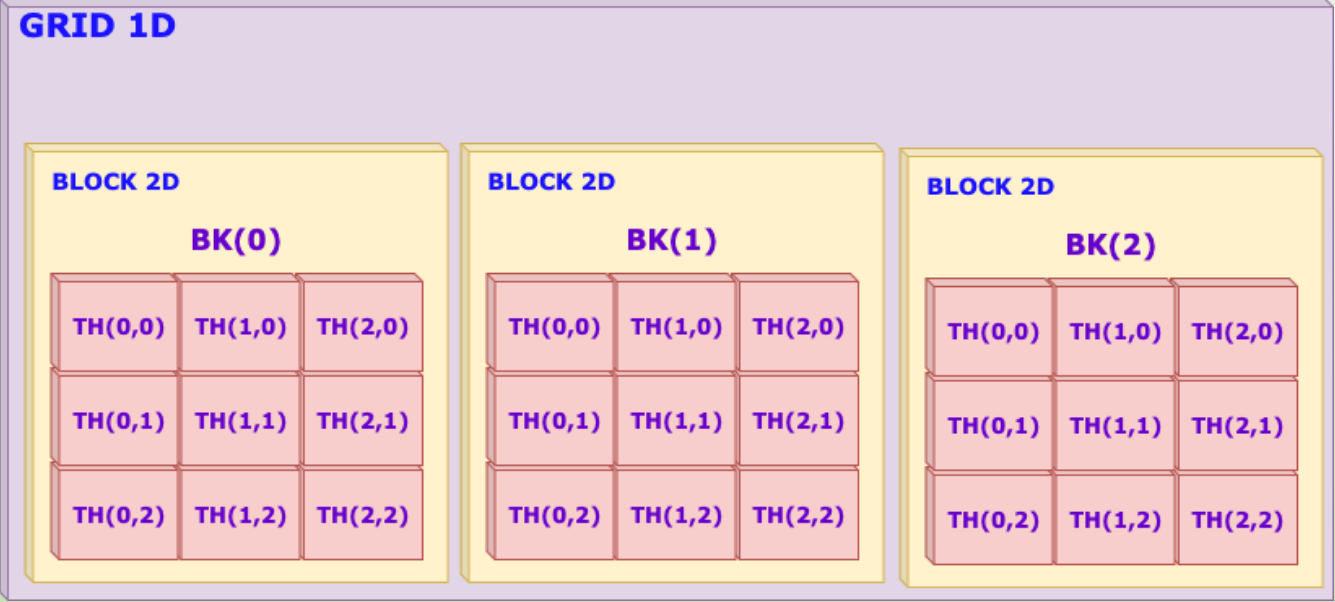
\includegraphics[width=0.98\linewidth]{img/cuda/grdiblock}
\end{center}

Tutti i blocchi devono essere uguali, in struttura e numero di thread. La griglia replica blocchi tutti uguali, ogni blocco ha thread uguali.

In qualsiasi caso, in \textbf{ogni blocco} ci possono essere \textbf{al più 1024 thread}; esempi di dimensioni: $(1024, 1, 1)$  o $(32, 16, 2)$, il totale non può superare 1024.\\

\paragraph{Thread block:} Un blocco di thread è un gruppo di thread che possono cooperare tra loro mediante:
\begin{itemize}
	\item Block-local synchronization
	\item Block-local shared memory
\end{itemize}

La memoria più veloce è condivisa solo dallo stesso blocco, quindi da CUDA 9.0 e CC 3.0+ thread di differenti blocchi possono cooperare come Cooperative Groups.\\

Tutti i thread in una grid condividono lo stesso spazio di global memory. Una grid rappresenta un processo, ogni processo lanciato dall'host ha una sua grid associata.\\

I thread vengono identificati univocamente dalle coordinate: 
\begin{itemize}
	\item \texttt{blockId} (indice del blocco nella grid)
	\item \texttt{threadId} (indice di thread nel blocco)
\end{itemize}
Sono variabili built-in, ognuna delle quali con 3 campi: \texttt{x,y,z}.\\

Dimensioni di blocchi e thread: le dimensioni di grid e block sono specificate dalle variabili built-in: 
\begin{itemize}
	\item \texttt{blockDim} (dimensione di blocco, misurata in thread)
	\item \texttt{gridDim} (dimensione della griglia, misurata in blocchi)
\end{itemize}
Sono di tipo \texttt{dim3}, un vettore di interi basato su \texttt{uint3}. I campi sono sempre \texttt{x,y,z}. Ogni componente non specificata è inizializzata a 1.\\

\paragraph{Linearizzare gli indici:} Ovviamente gli indici in blocchi a più dimensioni si possono linearizzare: con due indici $x,y$ posso unificarli facendo $x + y \cdot D_x$, dove $D_x$ è la dimensione della riga.\\
Possiamo tradurlo in un indice unico per i thread: per griglie e blocchi a 1D ciascuno: 
\begin{center}
	\texttt{IDth = blockIdx.x * blockDim.x + threadIdx.x}
\end{center}
Si può scalare a più dimensioni.\\

\paragraph{Lanciare un kernel:} Per lanciare un kernel CUDA si aggiungono tra triple parentesi angolari le dimensioni di grid e block.
\begin{center}
	\texttt{kernel\_name <<<grid, block>>>(argument list);}
\end{center}

\paragraph{Runtime API:} Alcune funzioni:
\begin{itemize}
	\item \texttt{cudaDeviceReset()} distrugge tutte le risorse associate al device per il processo corrente, non molto usato ma si può fare
	\item \texttt{cudaDeviceSynchronize()} aspetta che la GPU termini l'esecuzione di tutti i task lanciati fino a quel punto, sincronizzazione host device
\end{itemize}
Per effettuare debugging, la \texttt{Synchronize} permette di "scaricare" tutti i \texttt{printf} quando servono. Altrimenti, dato che le chiamate sono asincrone, si rischia che l'applicazione lato CPU termini prima che i \texttt{printf} abbiano avuto modo di essere mostrati. \\

Un altro mezzo di debugging è \texttt{Kernel<<<1,1>>>}: forza l'esecuzione su un solo blocco e thread, emulando comportamento sequenziale sul singolo dato.\\

Proprietà dei kernel: 
\begin{center}
	\begin{tabular}{| l | l | p{4cm} |}
		\hline
		\textbf{QUALIFICATORI} & \textbf{ESECUZIONE} & \textbf{CHIAMATA} \\
		\hline
		\texttt{\_\_global\_\_} & Eseguito dal device & Dall’host e dalla compute cap. 3 anche dal device \\
		\hline
		\texttt{\_\_device\_\_} & Eseguito dal device & Solo dal device \\
		\hline
		\texttt{\_\_host\_\_} & Eseguito dall’host & Solo dall’host \\
		\hline
	\end{tabular}
\end{center}

\paragraph{Restrizioni del kernel: }
\begin{itemize}
	\item Accede alla sola memoria device
	\item Deve restituire un tipo \texttt{void}
	\item Non supporta il numero variabile di argomenti
	\item Non supporta variabili statiche
	\item Non supporta puntatori a funzioni
	\item Esibisce un comportamento asincrono rispetto all'host
\end{itemize}

\paragraph{Gestione degli errori:} Si ha un \texttt{enum cudaError\_t} come valore di ritorno di ogni chiamata cuda. Può essere \texttt{success} o \texttt{cudaErrorMemoryAllocation}. Si può usare {cudaError\_t cudaGetLastError(void)} per ottenere il codice dell'ultimo errore.\\

%boh

%Misurare il tempo con la CPU
%smth smth

%Idk, I guess L2 is over, some lab in it

\newpage

\subsection{Warp}

\textbf{Ogni thread} vede: 
\begin{itemize}
	\item i suoi \textbf{registri privati}
	\item la \textbf{memoria condivisa} del blocco di thread
\end{itemize}
%Prime slide

Single Instruction Multiple Thread; l'architettura è basata sul \textbf{warp}, (tradotto in "trama" nella tessitura), l'idea è che ci sono delle file di thread (warp), collegate assieme dall'ordito. Rappresenta i blocchi di thread, sono blocchi da 32. Ogni Streaming Mutiprocessor SM esegue i thread in gruppi di 32, chiamati warp. Idealmente, tutti i thread in un warp eseguono la stessa cosa in parallelo allo stesso tempo (SIMD all'interno del warp).\\

Ogni thread ha il suo program counter e register state e può seguire cammini distinti di esecuzione delle istruzioni (parallelismo a livello thread, da Volta in poi, prima c'era un PC solo per ogni warp).\\

Il valore 32 è l'unità minima di esecuzione che permette grande efficienza nell'uso della GPU, concettualmente i blocchi di 32 dovrebbero avere modello SIMD, anche se nella pratica è SIMT (più flessibile ma potenzialmente meno efficiente). Dove si può si deve \textbf{evitare la divergenza di esecuzione} all'interno del warp. I \textbf{blocchi} vengono \textbf{divisi in warp}, quindi è meglio avere blocchi con thread multipli di 32, per evitare divergenza.\\

I blocchi di thread possono essere configurati logicamente in 1,2 o 3 dimensioni, ma a livello hardware sarà una sola dimensione con id progressivo, con un warp ogni 32 thread.\\

Sarà quindi necessario uno scheduling per i warp (il numero di blocchi richiesto è maggiore, chi va prima in esecuzione?) all'interno dei blocchi, vengono mandati in esecuzione quando sono liberi. Ad ogni colpo di clock lo scheduler dei warp decide quale mandare in esecuzione tra quelli che 
\begin{itemize}
	\item non sono in attesa di dati dalla device memory (alta latenza, memory latency)
	\item non stanno completando un'istruzione precedente (pipeline delay)
\end{itemize}
Questi dettagli sono trasparenti al programmatore, serve solo a garantire un elevato numero di warp in esecuzione; vogliamo massimizzare l'occupancy (percentuale di risorse usate in ogni SM) .\\

Se all'interno di un warp dei thread devono eseguire istruzioni diverse (e.g., per un \texttt{if}), la GPU le eseguirà sequenzialmente al posto che in parallelo, disabilitando i thread inattivi. Questa è una \textbf{divergenza} e riduce l'efficienza, a volte anche significativamente.  \\

Ogni warp ha un contesto di esecuzione (runtime), trasparente al programmatore, che consta di: 
\begin{itemize}
	\item Program counters
	\item Registri a 32-bit ripartiti tra thread
	\item Shared memory ripartita tra blocchi
\end{itemize} 

Di conseguenza, la memoria locale ad ogni thread è limitata, bisogna prestare attenzione alle risorse richieste simultaneamente per ogni thread, altrimenti il numero di thread che possono essere attivi in maniera concorrente si riduce.\\

I registri sono usati per le variabili locali automatiche scalari (che non sono array quindi) e le coordinate dei thread. I dati nei registri sono privati ai thread (scope) e ogni multiprocessor ha un insieme di 32-bit register che sono partizionati tra i warp.\\

%S17 scrivi
% Ma controlla un po' tutto tbh

Il numero di blocchi e warp che possono essere elaborati insieme su un SM per un dato kernel dipende
\begin{itemize}
	\item dalla quantità di registri e di shared memory usata dal kernel
	\item dalla quantità di registri e shared memory resi disponibili dallo SM
\end{itemize}
Ogni architettura ha i suoi vincoli e noi vogliamo avvicinarci il più possibile ai limiti massimi, in modo da rendere il più efficiente possibile il programma. C'è un numero massimo di thread/blocchi/warp per multiprocessor, vogliamo fare in modo di avere l'utilizzo maggiore possibile.\\

\newpage

%Latency hiding
\paragraph{Latency Hiding:} La "latenza"  è il numero di cicli necessari al completamento di un'istruzione. Per massimizzare il throughput occorre che lo scheduler abbia sempre warp eleggibili ad ogni ciclo di clock. Si ha così latency hiding intercambiando la computazione tra warp.\\
Tipi di istruzioni che inducono latenza: 
\begin{itemize}
	\item Istruzioni aritmetiche: tempo necessario per la terminazione dell'operazione (\texttt{add}, \texttt{mult}, \dots); 10-20 cicli di clock
	\item Istruzioni di memoria: tempo necessario al dato per giungere a destinazione (\texttt{load}, \texttt{store}); 400-800 cicli di clock
\end{itemize}
La griglia viene suddivisa in blocchi, il blocco in thread, i blocchi vanno all'SM.
\begin{center}
	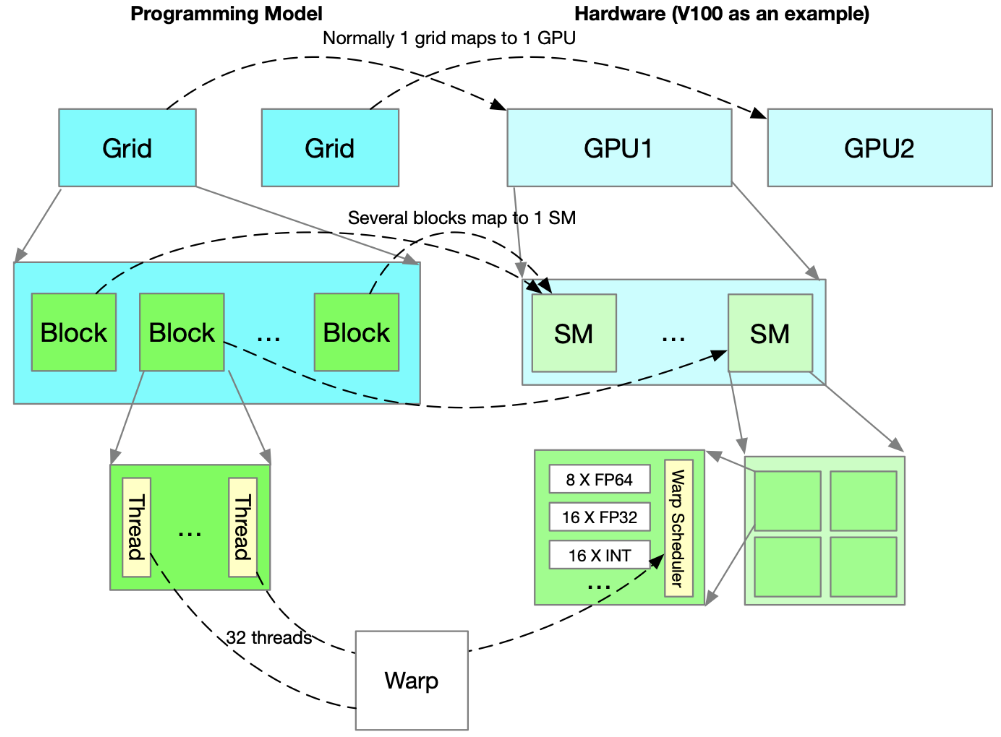
\includegraphics[width=0.85\linewidth]{img/cuda/modelandhwstruct}
\end{center}

%sincronizzazione smth up to s29

\newpage

\paragraph{Sincronizzazione a più livelli: } Le prestazioni decrescono con l'aumentare della divergenza nei warp. Primitive di sincronizzazione sono necessarie per evitare race conditions in cui diversi thread accedono simultaneamente alla stessa locazione di memoria. Si possono avere più livelli di sincronizzazione:
\begin{itemize}
	\item \textbf{System-level}: attesa che venga completato un dato task su entrambi host e device
	\begin{center}
		\texttt{cudaError\_t cudaDeviceSynchronize(void);}
	\end{center}
	Blocca l'applicazione host finché tutte le operazioni CUDA non sono completate;
	
	\item \textbf{Block-level}: attesa che tutti i thread in un blocco raggiungano lo stesso punto di esecuzione
	\begin{center}
		\texttt{\_\_device\_\_ void \_\_syncthreads(void);}
	\end{center}
	Sincronizza i thread all'interno di un blocco: attende fino a che tutti raggiungono il punto di sincronizzazione
	
	\item \textbf{Warp-level}: attesa che tutti i thread in un warp raggiungano lo stesso punto di esecuzione
	\begin{center}
		\texttt{\_\_device\_\_ void \_\_syncwarp(mask);}
	\end{center}
	Sincronizza i thread all'interno di un warp: attende fino a che tutti raggiungono il punto di sincronizzazione (riconverge)
\end{itemize}
La sincronizzazione a livello di blocco va usata con attenzione, può anche portare a deadlock, un esempio semplice può essere una sincronizzazione dentro un \texttt{if-else}, potrebbero esserci thread che non entreranno mai nel ramo con la sincronizzazione, deadlock.\\

Il compilatore ha tecniche di ottimizzazione per evitare divergenza all'interno del warp (es: per un if calcola entrambi i branch).\\

%manca boh, cazzo ne so
% Fino slide 37
% Resto lab

\newpage

\subsection{Memoria CUDA}

Per il programmatore esistono due tipi di memorie: 
\begin{itemize}
	\item \textbf{Programmabile}: controllo esplicito di lettura e scrittura per dati che transitano in memoria
	\item \textbf{Non programmabile}: nessun controllo sull'allocazione dei dati, gestiti con tecniche automatiche (es. memorie CPU e cache L1 e L2 della GPU)
\end{itemize}

Nel modello di memoria CUDA sono esposti diversi tipi di memoria programmabile: 
\begin{enumerate}
	\item registri
	\item shared memory
	\item local memory
	\item constant memory
	\item texture memory
	\item global memory
\end{enumerate}

\paragraph{Cache su GPU:} Come nel caso delle CPU, le cache su GPU \textbf{non sono programmabili}. Sono presenti 4 tipi:
\begin{itemize}
	\item \textbf{L1}, una per ogni SM
	\item \textbf{L2}, condivisa tra tutti gli SM
	\item \textbf{Read-only constant}
	\item \textbf{Read-only texture} (L1 da cc 5.0)
\end{itemize}

La cache L1 è presente all'interno di ogni SM; in alcune architetture (Fermi e successive) la dimensione può essere configurata, con una porzione assegnabile a memoria condivisa. Capacità limitata ma permette di sfruttare località dei dati.\\
La cache L2 ha dimensione maggiore ed è condivisa tra tutti gli SM, funziona da intermediario tra memoria globale e cache L1 dei singoli SM. Raccoglie i dati necessari a tutti gli SM e contribuisce a mantenere la coerenza dei dati tra vari SM.\\

L1 e L2 sono usate per memorizzare dati in memoria locale e globale, incluso lo spilling dei registri (eccessi nell'uso di local memory). \\

Ogni SM ha anche una read-only constant cache e read-only texture cache (non sempre fisiche) usate per migliorare le prestazioni in lettura dai rispettivi spazi di memoria sul device. \\

Read-only constant cache è ottimizzata per dati globali costanti condivisi tra tutti i thread, con accesso uniforme e caching efficiente. Read-only texture cache è ideale per dati in sola lettura con accesso non coalescente, sfruttando la località spaziale e offrendo funzionalità di interpolazione e filtraggio hardware. \\

Suddivisione fisica:
\begin{center}
	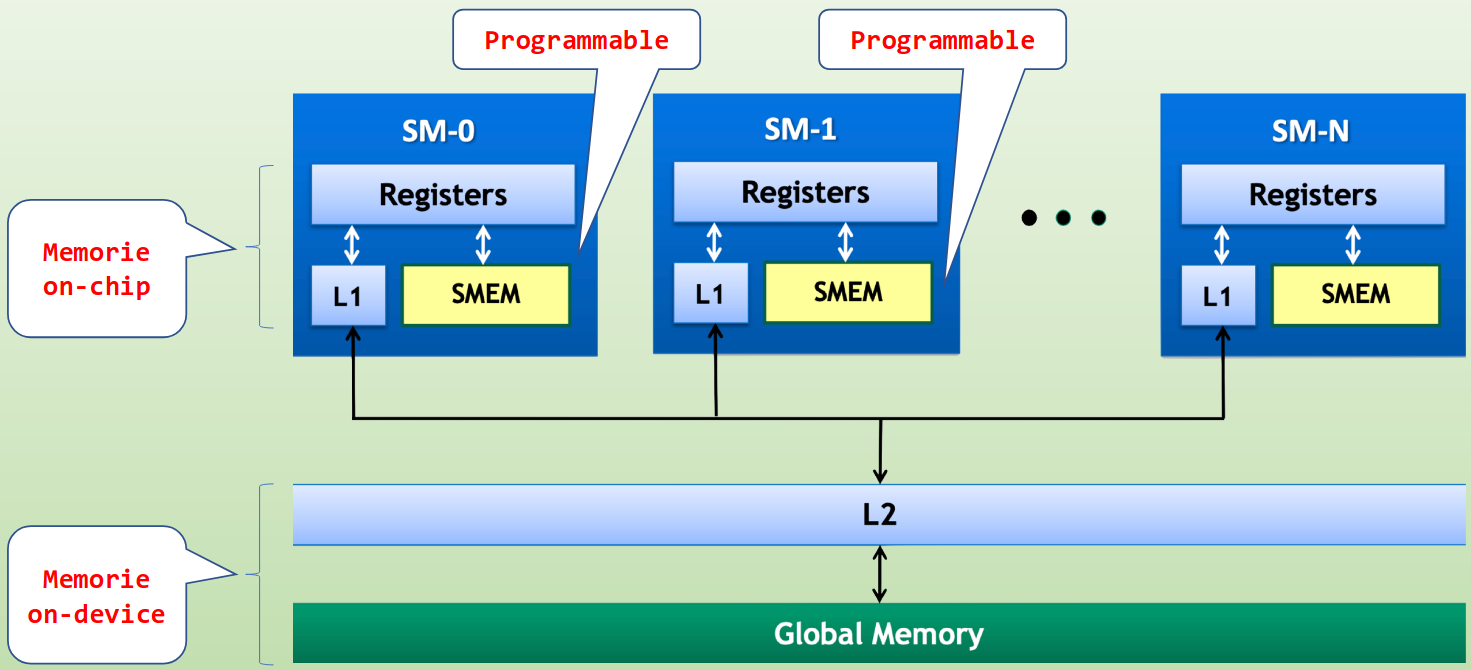
\includegraphics[width=0.9\linewidth]{img/cuda/mem1}
\end{center}

Nel tempo, è stata gradualmente aumentata la dimensione delle cache L1 e L2, allo stesso tempo incrementando la memoria condivisa tra gli SM, fino all'introduzione di una L0 instruction cache in Volta, oltre a 128kB di cache L1 unita alla shared memory (smem).\\

\newpage

\subsubsection{Cooperating Threads/Shared Memory}
Un blocco può avere della memoria condivisa e tutti thread all'interno del blocco hanno la stessa visuale su questa memoria; la memoria è unica per blocco ed inaccessibile ad altri blocchi. Viene dichiarata tramite \texttt{\_\_shared\_\_}.\\

La SMEM è suddivisa in moduli della stessa ambiezza, chiamati \textbf{bank}. Ogni richiesta di accesso fatta di $n$ indirizzi che riguardano $n$ distinti bank sono serviti simultaneamente.\\

Ogni SM ha una quantità limitata di shared memory che viene ripartita tra i blocchi di thread. La smem serve come base per la comunicazione inter-thread: i thread all'interno di un blocco possono cooperare scambiandosi dati memorizzati in shared memory. L'accesso deve essere sincronizzato per mezzo di \texttt{syncthreads()}.\\

\paragraph{Organizzazione fisica:} La smem è suddivisa in blocchi da 4 byte (word), ogni accesso legge almeno la word di appartenenza (anche se viene richiesto un solo byte).\\

Dati 32 bank, ogni word è memorizzata in bank distinti, a gruppi di 32. Dato l'indirizzo del byte: 
\begin{itemize}
	\item diviso 4 si ottiene l'indice della word
	\item l'indice della word modulo $32$ è l'indice della bank
\end{itemize}

\paragraph{Smem a runtime:} La memoria viene ripartita tra tutti i blocchi residenti in un SM. Maggiore è la shared memory richiesta da un kernel, minore è il numero di blocchi attivi concorrenti. Il contenuto della shared memory ha lo stesso lifetime del blocco a cui è stata assegnata.\\

\newpage

\paragraph{Pattern di accesso:} Se un'operazione di load o store eseguita da un warp richiede al più un accesso per bank, si può effettuare in una sola transizione il trasferimento dei dati dalla shared memory al warp. In alternativa sono richieste diverse ($\leq 32$) transazioni, con effetti negativi sulla bandwidth globale.\\

L'accesso ideale è una singola transazione per warp.\\

Ci possono essere dei \textbf{conflitti}: un \textbf{bank conflict} accade quando si hanno diversi indirizzi di shared memory che insistono sullo stesso bank.\\
L'hardware effettua tante transazioni quante ne sono necessarie per eliminare i conflitti, diminuendo la bandwidth effettiva di un fattore pari al numero di transazioni separate necessarie (vengono serializzati gli accessi).\\

\paragraph{Osservazioni:}
\begin{itemize}
	\item \textbf{Latency hiding}: il ritardo tra richiesta dei thread alla smem e l'ottenimento dei dati non è in generale un problema, anche in caso di bank conflict; lo scheduler passa ad un altro warp in attesa che quelli sospesi completino il trasferimento dei dati dalla smem
	\item \textbf{inter-block}: non esiste conflitto tra thread appartenenti a blocchi differenti, il problema sussiste solo a livello di warp dello stesso blocco 
	\item \textbf{Efficienza massima}: il modo più semplice per avere prestazioni elevate è quello di fare in modo che un warp acceda a word consecutive in memoria shared
	\item \textbf{Caching}: con lo scheduling efficace, le prestazioni (anche in presenza di conflitti a livello smem) sono molto migliori rispetto alla cache L2 o global memory
\end{itemize}

\newpage

\subsubsection{Allocazione della SMEM}

\paragraph{Allocazione statica:} Una variabile in shared memory può anche essere dichiarata locale a un kernel o globale in un file sorgente. Viene dichiarata con il qualificatore \texttt{\_\_shared\_\_}. Può essere dichiarata sia staticamente sia dinamicamente. Se statica, può essere 1D, 2D o 3D, con dimensione nota compile time.\\
Dinamicamente si possono allocare solo array 1D.\\

Se la dimensione non è nota compile time, è possibile dichiarare una variabile adimensionale con la keyword \texttt{extern}.\\

\paragraph{Allocazione dinamica:} Per allocare la shared memory dinamicamente (in bytes), occorre indicare un terzo argomento all'interno della chiamata del kernel:
\begin{center}
	\texttt{kernel <<<grid, block, N*sizeof(int)>>>(\dots)}
\end{center}

%TODO completa slide 27-28


